\chapter{Introduction}
\label{chap-intro}

Physics is to study matters of the universe where 
there are tremendous more disordered materials than ordered ones.
In ordered physics, there has been a rich spectrum of 
well-defined theories, models, phases, and methods; while disordered 
systems still have a variety of challenging and unclear questions. 

This chapter first introduces the general disordered system and 3 specific disordered systems, i.e. jamming transition, antiferromagnetic Ising model, and random field Ising model. Then the finite dimensional networks we use in our study are explained. In the end of this chapter, the existing work of disordered system in complex networks is reviewed to understand the problem and how we can contribute new insights.  

\section{Disordered System}
In real world, most materials can be considered as disordered materials because of the heterogeneous structures with defects and impurities. There are various types of disordered materials, such as glass\cite{Gibbs1958nature}, amorphous solids \cite{berthier2016facets}, polymer \cite{roth2005glass}, granular material \cite{richard2005slow}, and biological tissue \cite{bi2015density}. 

Here we focus on models of disordered systems that lend themselves to theoretical investigations, such as Edwards-Anderson model \cite{edwards1975theory}, random field Ising model \cite{imry1975random}, antiferromagnetic Ising model\cite{wannier1950afm},  fully frustrated model \cite{kosterlitz1973ordering, kosterlitz1974critical}, spin glass \cite{young1997spin}, lattice glass model \cite{Biroli02}. 

To Be Completed later!

BLANK.\footnote{This will be changed!}

\section{Jamming Transition}
\label{sec:jam_intro}
The first focus here is on the jamming systems \cite{Biroli2007}. Those systems undergo 
a jamming transition from a liquid-like to a solid-like state with extremely slow 
dynamics at a high packing density. The most interesting part in this 
disordered system is the physics near the jamming transition. 
The jamming transition, as discussed by Liu and
Nagel in 1998~\cite{Liu1998} has been the focus of
intense study~\cite{Biroli2007,Liu2010,Berthier2011}. 

A granular disordered system with increasing density can reach a jammed state at which a finite yield stress develops, or at least extremely long relaxation times
ensue, similar to the emerging sluggish behavior observed when the
viscosity of a cooled glassy liquid seemingly diverges. Thus, a jamming
transition may be induced in various ways, such as by increasing density,
decreasing temperature, or/and reducing shear stress~\cite{Liu2010}.
Below the jamming transition, the system stays in long-lived meta-stable
states, and its progression to its corresponding equilibrium state
entails an extremely slow, non-Debye relaxation~\cite{Hill1985,Ciamarra2010,van2010}.

Jamming transitions have been observed in various types of systems,
such as granular media~\cite{Majmudar2007}, molecular glasses~\cite{Parisi2010,Angelani2007},
colloids~\cite{Trappe2001}, emulsions~\cite{Zhang2005}, foams~\cite{Berthier2011,DaCruz2002},
etc~\cite{Liu2010,van2010}. These systems can behave like stiff solids
at a high density with low temperature and small perturbations. In
these transitional processes, the systems can self-organize their
own structure to avoid large fluctuations~\cite{Berthier2011} and
to reach a quasi-stable jammed state, characterized by an extremely
slow evolution to the unjammed equilibrium state. The properties of
those quasi-stable non-equilibrium states as well as their corresponding
equilibrium state is the main focus of our work in jamming. 


The properties of the jamming transition have been studied 
extensively~\cite{Biroli2007,Majmudar2007,Liu2010}, but we still lack an essential
understanding of the physics underlying the jammed state. Theoretical
progress has been much slower than the accumulation of experimental
discoveries. One of the reasons is the scarcity of theoretical microscopic
models to capture the complex jamming process~\cite{Krzakala2008,Jacquin2011}. 

In recent years, a lattice glass model proposed by Biroli and Mezard
(BM)~\cite{Biroli02} has been shown as a simple but adequate means
to study the jamming process. It is simple because the model follows
specific dynamical rules which are elementary to implement in both
simulations and analytical work. In distinction to kinetically constrained
models such as that due to Kob and Andersen~\cite{Kob93}, in which
particles are blocked from leaving a position unless certain neighborhood
conditions are satisfied, BM embeds geometric frustration merely by
preventing the neighborhood of any particles to consist of more than
$l$ other particles. Beyond that, it proceeds purely thermodynamically.
The phase diagram can be reduced to just one (or both) of two control
parameters, chemical potential and temperature. Either is sufficient
to reproduce a jamming transition which is similar to that observed
in off-lattice systems~\cite{Biroli02}. 

Using this model in a mean-field network 
(i.e., a regular random graph), Krzakala \textit{et al.} find
jammed states in Monte Carlo simulations and a genuine thermodynamical
phase transition (ideal glass transition) in its mean-field analytical
solutions~\cite{Krzakala2008}. In other words, the jammed state coincides
with an underlying equilibrium state that possesses a phase transition
to a glassy state. There is also other work trying to prove the similar idea using mean-field models \cite{Rivoire03,berthier2011theory, Parisi2010}. That raises the prospect that this equilibrium phase transition might be the reason for the onset of jamming. However, such a connection between phase transition and jamming transition is hard to ascertain for finite-dimensional lattice glasses. Our work (Chapter \ref{chap-jamming}) focuses on jamming in finite-dimensional hierarchical networks which could contribute closer insights to real world systems.

\section{Ising models}
\subsection{Antiferromagnetic Ising Model}
\label{sec:intro-afm}
abc

\subsection{Random Field Ising Model}
\label{sec:intro-rfim}
cddf

\section{Hanoi Networks}
\label{sec:HN} 
In our investigations, one of the innovative insights is contributed from the finite-dimensional lattice-like networks. We use 4 types of Hanoi networks ~\cite{Boettcher2008HN} which are small-world networks with a hierarchical, recursive structure that avoid the usual randomness involved in defining
an ensemble of networks. Thus, no additional averages of such an ensemble
are required to obtain scaling properties in thermodynamical limit
from a finite system size, which reduces the computational effort.
Hanoi networks combine a real-world geometry with a hierarchy of small-world
links, as an instructive intermediary between mean-field and finite-dimensional
lattice systems, on which potentially exact results can be found using
the renormalization group~\cite{BoHa11}. 

Across all the chapters, we use four Hanoi networks: HN3, HN5, HNNP, and HN6. Their general characteristics are summarized in Table \ref{tab:hns}.

\begin{table}
\begin{centering}
\protect\caption{\label{tab:hns} 
Summary of Hanio networks at system size $N\rightarrow\infty$ }
\par\end{centering}
\begin{centering}
\par\end{centering}
\centering{}%
\begin{tabular}{|c|c|c|c|c|}
\hline 
Network & Degree  & Planarity & Diameter & Fractal Dimension  \tabularnewline
\hline 
\hline 
HN3  & 3 & Planar & $\sqrt{N}$ & 2 \tabularnewline
\hline 
HN5  & 5 & Planar &  $\ln N$ & $\infty$  \tabularnewline
\hline 
HNNP  & 4  & Nonplanar &  - & -  \tabularnewline
\hline 
HNNP  & 6  & Nonplanar &  - & - \tabularnewline
\hline 
\end{tabular}
\end{table}

Each of them can be built on
a simple backbone of a 1D lattice. The 1D backbone has $N=2^{k}+1$
($k=1,2,3,\cdots$) sites where each site is numbered from $0$ to
$N$. Any site $n$, $0\le n\le N$, can be defined by two unique
integers $i$ and $j$, 
\begin{equation}
n(i,j)=2^{i-1}(2j+1),\label{eq:numbering}
\end{equation}
where $i$, $1\le i\le k$, denotes the level in the hierarchy and
$j$, $0\le j<2^{k-i}$, labels consecutive sites within each
hierarchy $i$. Site $n=0$ is defined in the highest level $k$ or,
equivalently, is identified with site $n=N$ for periodic boundary
conditions. With this setup, we have a 1D backbone of degree
2 for each site and a well-defined hierarchy on which we can build
long-range links recursively in three different ways: HN3~\cite{Boettcher2008HN}
is constructed by connecting the neighbor sites $n(i,0)\longleftrightarrow n(i,1)$,
$n(i,2)\longleftrightarrow n(i,3)$, $n(i,4)\longleftrightarrow n(i,5)$,
and so on and so forth. For example, in level $i=1$, site $n(1,0)=1$
is connected to $n(1,1)=3$; site $n(1,2)=5$ is connected to $n(1,3)=7$;
and so on. A initial section of a HN3 network is given in Fig.~\ref{fig:HN3_short}.
As a result, HN3 is a planar network of regular degree 3.

\begin{figure}
\centering 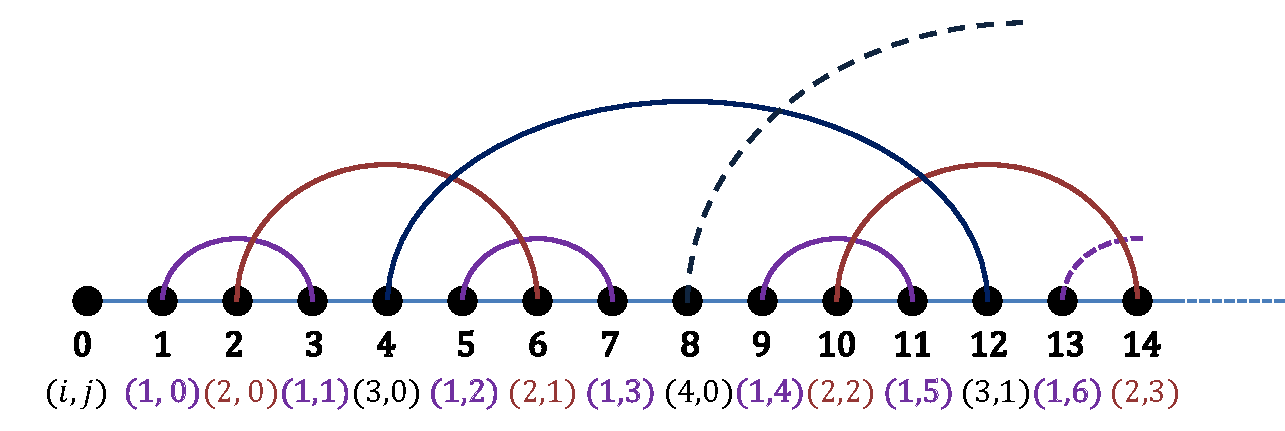
\includegraphics[width=1\columnwidth]{Chapter-1/HN3_short.pdf} 
\protect\caption{\label{fig:HN3_short} An example of the first 14 sites of HN3 on a semi-infinite line.}
\end{figure}




HN5~\cite{Boettcher09c}, as shown in Fig.~\ref{fig:Depiction-of-HN},
is an extension based on HN3, where each site in level $i$ ($i\ge2$,
i.e., all even sites) is further connected to sites that are $2^{i-1}$
sites away in both directions. For example, for the level $i=2$ sites
(sites $2,6,10,\cdots$), site 2 is connected to both site 0 and site
4; site 6 is connected to sites 4 and 8; etc. The resulting network
remains planar but has a hierarchy-dependent degree, i.e., 1/2 sites
have degree 3, 1/4 have degree 5, 1/8 have degree 7, etc. In the limit
of $N\to\infty$, this network has  average degree 5.

\begin{figure}
\centering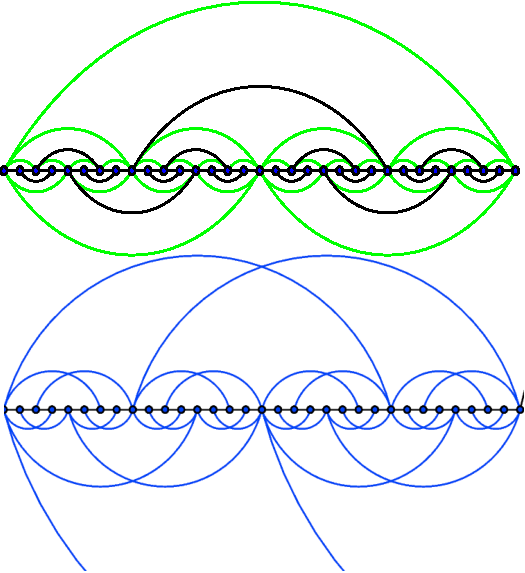
\includegraphics[width=0.8\columnwidth]{Chapter-1/HN5HNNP}
\protect\caption{\label{fig:Depiction-of-HN}Depiction of HN5 (top) and HNNP (bottom),
first introduced in Ref. \protect\cite{Boettcher09c}. Green-shaded lines
in HN5 represent its difference to HN3, which is at its core (dark
lines). While HN3 and HN5 are planar, HNNP is non-planar. }
\end{figure}

HNNP~\cite{Boettcher09c}, also shown in Fig.~\ref{fig:Depiction-of-HN},
is constructed from the same 1D backbone as HN3 and HN5. However,
for site $n$ in level $i$ with even $j$, it is connected forwards
to site $(n+3\times2^{i-1})$; while site $n$ in level $i$ with
odd $j$ is connected backwards to site $(n-3\times2^{i-1})$. Level
1 and level 2 sites have degree 3, and level $3,4,5,\cdots$ sites
have degree $5,7,9,\cdots$. The HNNP has an average degree of 4 and
is non-planar.

HN6 \cite{Boettcher09c} is constructed from HNNP in the same way of constructing HN5 from HN3. The extra links are initiated from site in level $i$ ($i\ge2$ who
i.e., all even sites)  connects to sites that are $2^{i-1}$
sites away in both directions. The resulting network is still a nonplanar with hierarchy-dependent degree.

As you can see, these four networks are all constructed hierarchically and can potentially use renormalization group in a similar way. Using these networks, renormalization group has been applied to lattice gas model \cite{cheng2015jamming, BoHa11} and ferromagnetic Ising model \cite{Boettcher2011HNNP, boettcher2015classification}. In the study here, the models are extended to lattice glass model and antiferromagnetic Ising model. 




\section{Computational Methods}

Wang-Landau sampling is a computational methods using non-Markov-chain Monte Carlo; while RG is an analytical methods but requires the computational implementation using modern symbolic computational tools (Mathematica.)
